\section{Introducción a las Bases de Datos}



\begin{ejercicio}\label{ej:4.Ejercicio1}
    Se desea diseñar un esquema relacional de una base de datos para un centro de enseñanza que contenga información sobre los alumnos (dni, nombre, dirección \dots), las asignaturas (código de asignatura y nombre de esta se considera la información mínima) y las calificaciones que se obtienen en cada una de las mismas. Desarrollar un modelo ER del mismo y posteriormente reducirlo a tablas.

    \begin{figure}[H]
        \centering
        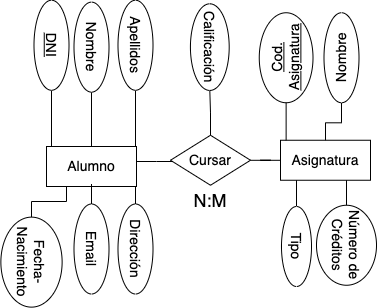
\includegraphics[width=0.6\linewidth]{Imagenes/Ejercicio 1.png}
        \caption{Modelo Entidad-Relación del ejercicio \ref{ej:4.Ejercicio1}}
        \label{fig:Ej1}
    \end{figure}


    Tendríamos tres tablas:
    \begin{description}
        \item [Alumno] (\underline{DNI}, Nombre, Apellidos, Dirección, Email, Fecha de Nacimiento)

        \item [Asignatura] (\underline{Cód-Asignatura}, Nombre, Tipo, Número de Créditos)

        \item [Cursar] (\underline{DNI}, \underline{Cód. Asignatura}, Calificación)
    \end{description}
\end{ejercicio}

\newpage
\begin{ejercicio} \label{ej:4.Ejercicio2}
Se desea diseñar la base de datos de una biblioteca particular, de modo que para cada libro se deberá almacenar: su título, número de páginas, ISBN, materia, año de edición, editorial y autor o autores del mismo, para los que, además de su nombre, se recogerán los siguientes datos: dirección de correo electrónico, nacionalidad y fecha de nacimiento. Además, para cada editorial se deberá guardar su dirección, localidad y país. Teniendo en cuenta que se pueden añadir los campos que se consideren oportunos para poder relacionar convenientemente las distintas entidades del problema, realizar lo que se pide en cada uno de los siguientes apartados:
\begin{itemize}
    \item Dibujar el esquema conceptual, utilizando el modelo entidad-relación.
    \begin{figure}[H]
        \centering
        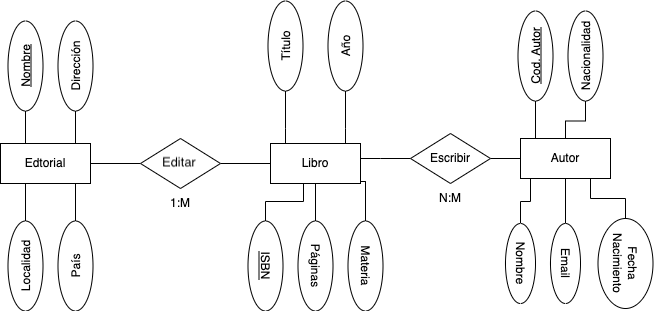
\includegraphics[width=0.8\linewidth]{Imagenes/Ejercicio 2.png}
        \caption{Modelo Entidad-Relación del ejercicio \ref{ej:4.Ejercicio2}}
        \label{fig:Ej2}
    \end{figure}
    
    \item Obtener, a partir de lo realizado en el apartado anterior, las tablas que se tendrían que crear en un SGBD relacional, indicando qué campos compondrían cada tabla y cuál sería la clave primaria de cada una de ellas.

    Tendríamos cuatro tablas:
    \begin{description}
        \item [Autor] (\underline{Cod. Autor}, Nombre, Email, FechaNacimiento, Nacionalidad)

        \item [Libro] (\underline{ISBN}, Título, Páginas, Materia, Año, NombreEd.)

        \item [Editorial] (\underline{NombreEd.}, Direcciones, Localidad, País)

        \item [Escribir] (\underline{Cod. Autor}, \underline{ISBN})
    \end{description}
\end{itemize}
\end{ejercicio}

\newpage
\begin{ejercicio}\label{ej:4.Ejercicio3}
Suponga que la base de datos para una Universidad del ejercicio (1) considera además de la información sobre los alumnos y las asignaturas, las carreras que se pueden estudiar. Construir un modelo ER y pasarlo posteriormente a un esquema relacional teniendo en cuenta las siguientes restricciones:
\begin{itemize}
    \item Un alumno puede estar matriculado en muchas asignaturas.
    \item Una asignatura sólo puede pertenecer a una carrera.
    \item Una carrera puede tener muchas asignaturas.
\end{itemize}

    \begin{figure}[H]
        \centering
        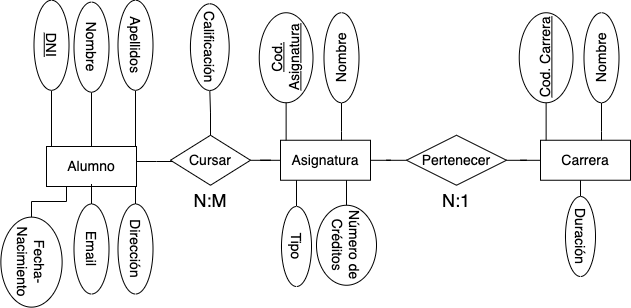
\includegraphics[width=0.8\linewidth]{Imagenes/Ejercicio 3.png}
        \caption{Modelo Entidad-Relación del ejercicio \ref{ej:4.Ejercicio3}}
        \label{fig:Ej3}
    \end{figure}


    Tendríamos tres tablas:
    \begin{description}
        \item [Alumno] (\underline{DNI}, Nombre, Apellidos, Dirección, Email, Fecha de Nacimiento)

        \item [Asignatura] (\underline{Cód. Asignatura}, Nombre, Tipo, Número de Créditos, Cód. Carrera)

        \item [Carrera] (\underline{Cód. Carrera}, Nombre, Duración)

        \item [Cursar] (\underline{DNI}, \underline{Cód. Asignatura}, Calificación)
    \end{description}

    \begin{observacion}
        Se podría considerar que el nombre de titulación fuese el campo llave.
    \end{observacion}
    
\end{ejercicio}


\newpage
\begin{ejercicio}\label{ej:4.Ejercicio4}
Se desea diseñar una base de datos para un centro comercial organizado por secciones que contenga información sobre los clientes que han comprado algo, los trabajadores, el género que se oferta y las ventas realizadas. Construir un modelo ER y pasarlo posteriormente a un esquema relacional teniendo en cuenta las siguientes restricciones:
\begin{itemize}
    \item Existen tres tipos de trabajadores: gerentes, jefes y vendedores.
    \item Cada sección está gestionado por un gerente.
    \item Un determinado producto sólo se encuentra en una sección.
    \item Los jefes y vendedores sólo pueden pertenecer a una única sección.
    \item Un gerente tiene a su cargo a un cierto número de jefes y éstos a su vez a un cierto número de vendedores.
    \item Una venta la realiza un vendedor a un cliente y debe quedar constancia del artículo vendido. Sólo una unidad de cada artículo por apunte de venta.
\end{itemize}

    \begin{figure}[H]
        \centering
        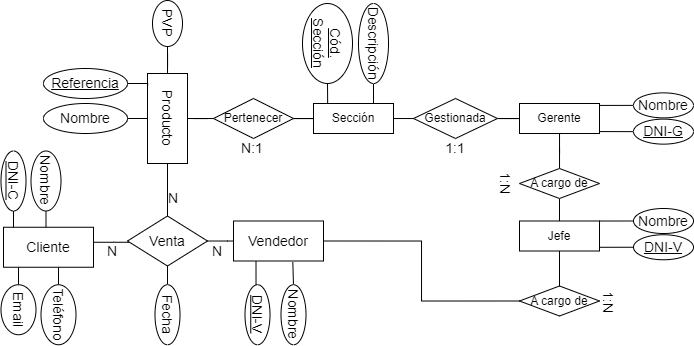
\includegraphics[width=0.8\linewidth]{Imagenes/Ejercicio 4.png}
        \caption{Modelo Entidad-Relación del ejercicio \ref{ej:4.Ejercicio4}}
        \label{fig:Ej4}
    \end{figure}

    Tendríamos las siguientes tablas:
    \begin{description}
        \item [Producto] (\underline{Referencia}, Nombre, PVP, Cód-Sección)
        \item [Sección] (\underline{Cód. Sección}, Descripción)
        \item [Gerente] (\underline{DNI-G}, Nombre, Cód-Sección)
        \item [Jefe] (\underline{DNI-J}, Nombre, DNI-G)
        \item [Vendedor] (\underline{DNI-V}, Nombre, DNI-J)
        \item [Comprador] (\underline{DNI-C}, Nombre, Teléfono, Email)
        \item [Venta] (\underline{Fecha}, \underline{DNI-C}, \underline{DNI-V}, \underline{Referencia})
    \end{description}

    \begin{observacion}
        En la tabla \textbf{Venta}, el campo Fecha sería clave o no si consideramos que la misma venta se puede repetir en fechas distintas.
    \end{observacion}
\end{ejercicio}


\newpage
\begin{ejercicio}\label{ej:4.Ejercicio5} \textbf{(EXAMEN)}
    Se desea implementar un sistema de gestión de cupones de la ONCE en el que se registre cada venta de cupones. En el caso de que un cupón resulte premiado, el comprador ha de acudir a una Administración a cobrarlo. Tenga en cuenta las siguientes restricciones:
    \begin{itemize}
        \item Cada cupón es único.
        \item Cada vendedor tiene asociado su código de la seguridad social.
        \item Cada comprador puede comprar más de un cupón y a distintos vendedores.
        \item Existe una única administración por provincia.
    \end{itemize}

    \begin{figure}[H]
        \centering
        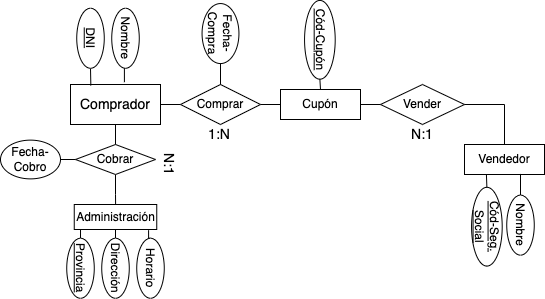
\includegraphics[width=0.8\linewidth]{Imagenes/Ejercicio 5.png}
        \caption{Modelo Entidad-Relación del ejercicio \ref{ej:4.Ejercicio5}}
        \label{fig:Ej5}
    \end{figure}

    Tendríamos las siguientes tablas:
    \begin{description}
        \item [Vendedor] (\underline{Cód-Seguridad Social}, Nombre)
        \item [Cupón] (\underline{Cód-Cupón}, Cód-Sedguridad Social)
        \item [Comprador] (\underline{DNI}, Nombre)
        \item [Comprar] (\underline{DNI}, \underline{Cód-Cupón}, Fecha-Compra)
        \item [Administración] (\underline{Provincia}, Dirección, Horario)
        \item [Cobrar] (\underline{Provincia}, \underline{DNI}, Fecha-Cobro)       
    \end{description}


\end{ejercicio}




\newpage
\begin{ejercicio}\label{ej:4.Ejercicio6}
    Los profesores de la asignatura de Bases de Datos de una Escuela Universitaria deciden crear una base de datos que contenga la información de los resultados de las pruebas realizadas a los alumnos. Para realizar el diseño, se sabe que:
    \begin{itemize}
        \item Los alumnos están definidos por su número de matrícula, nombre y grupo al que asisten a clase.
        \item Dichos alumnos realizan dos tipos de pruebas a lo largo del curso académico:
        \begin{enumerate}
            \item Exámenes escritos: cada alumno realiza varios a lo largo del curso, y se definen por el número de examen, el número de preguntas que que consta y la fecha de realización (la misma para todos los que realizan el mismo examen). Evidentemente, es importante almacenar la nota de cada alumno por examen.

            \item Prácticas: se realiza un número indeterminado de ellas durante el curso académico, algunas serán en grupo y otras individuales. Se definen por un código de la práctica, título y el grado de dificultad. En este caso, los alumnos pueden examinarse de cualquier práctica cuando lo deseen, debiéndose almacenar la fecha y la nota obtenida.
        \end{enumerate}

        \item En cuanto a los profesores, únicamente interesa conocer (además de sus datos personales: DNI y nombre), quién es el que ha diseñado cada práctica, sabiendo que en el diseño de una práctica puede colaborar más de uno, y que un profesor puede diseñar más de una práctica. Interesa, además, la fecha en que ha sido diseñada cada práctica por el profesor correspondiente.
    \end{itemize}

    Para ello se pide:
    \begin{enumerate}
        \item Diseñar un modelo Entidad Relación para este caso.

        \begin{figure}[H]
            \centering
            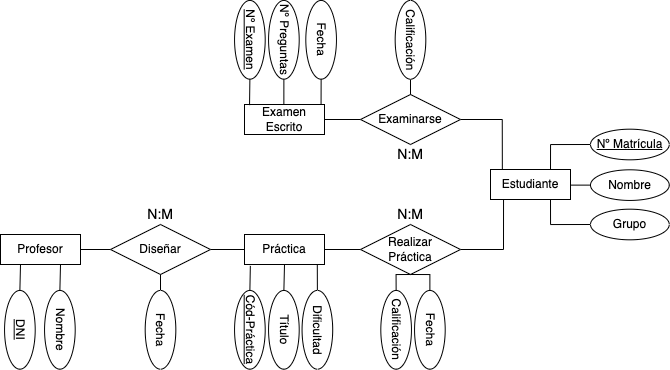
\includegraphics[width=0.8\linewidth]{Imagenes/Ejercicio 6.png}
            \caption{Modelo Entidad-Relación del ejercicio \ref{ej:4.Ejercicio6}}
            \label{fig:Ej6}
        \end{figure}

        \item Obtener, a partir de lo realizado en el apartado anterior, las tablas que se tendrían que crear en un SGBD relacional, indicando qué campos compondrían cada tabla y cuál sería la clave primaria para cada una de ellas.

        Tendríamos las siguientes tablas:
        \begin{description}
            \item [Profesor] (\underline{DNI}, Nombre)
            \item [Diseñar] (\underline{Cód-Práctica}, \underline{DNI}, Fecha)
            \item [Práctica] (\underline{Cód-Práctica}, Título, Dificultad)
            \item [Realizar Práctica] (\underline{Cód-Práctica}, \underline{Nº Matrícula}, Fecha, Calificación)
            \item [Estudiante] (\underline{Nº Matrícula}, Nombre, Grupo)
            \item [Examinarse] (\underline{Nº Matrícula}, \underline{Nº Examen}, Calificación)
            \item [Examen] (\underline{Nº Examen}, Nº de preguntas, Fecha)
        \end{description}
    \end{enumerate}

    

    


\end{ejercicio}




\newpage
\begin{ejercicio}\label{ej:4.Ejercicio7}
    Se desea diseñar un esquema relacional de una base de datos para un colegio mayor que represente que los residentes (DNI, edad, nombre, apellidos) tienen un responsable asignado (DNI, nombre, apellidos, dirección, móvil, parentesco) desde una determinada fecha para que el director de la residencia pueda contactar con ellos
    en caso de incidencias. Un residente puede tener un único tutor asignado y un tutor
    solo puede ser responsable de un alumno.

    Para ello se pide:
    \begin{enumerate}
        \item Diseñar un modelo Entidad Relación para este caso.

        \begin{figure}[H]
            \centering
            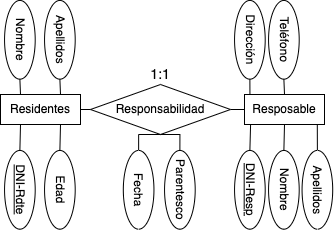
\includegraphics[width=0.5\linewidth]{Imagenes/Ejercicio 7.png}
            \caption{Modelo Entidad-Relación del ejercicio \ref{ej:4.Ejercicio7}}
            \label{fig:Ej7}
        \end{figure}

        \item Obtener, a partir de lo realizado en el apartado anterior, las tablas que se tendrían que crear en un SGBD relacional, indicando qué campos compondrían cada tabla y cuál sería la clave primaria para cada una de ellas.

        Tendríamos las siguientes tablas:
        \begin{description}
            \item [Residente] (\underline{DNI-Rdte}, Nombre, Apellidos, Edad)
            \item [Responsable] (\underline{DNI-Resp}, Nombre, Apellidos, Dirección, Teléfono)
            \item [Responsabilidad] (\underline{DNI-Rdte}, {DNI-Resp}, Fecha, Parentesco)
        \end{description}

        \begin{observacion}
            Hemos supuesto que un residente tiene el mismo responsable durante toda su estancia, que no puede cambiarlo.

            En el caso de que un residente pudiese cambiar de responsable, la cardinalidad sería 1:N, y el campo llave de la tabla responsabilidad sería 
            DNI-Resp o ambos DNIs, a elección.
        \end{observacion}
    \end{enumerate}

    

    


\end{ejercicio}